%latex slides_FMeot.tex  ; latex slides_FMeot.tex  ; dvips slides_FMeot.dvi ; dvipdf slides_FMeot.dvi 
\documentclass[12pt]{article}

%\usepackage{draftcopy}
%\usepackage[draft]{graphicx}
\usepackage{graphicx}
%\usepackage{wrapfig}
\usepackage{amssymb}
\usepackage{lscape}
\usepackage{times}
\usepackage{color}  % For \textcolor and \color % Ex. : \textcolor{red}{Text colored with} ; {\color{red}Text colored with}
\usepackage{soul}   % For \hl{ highlighted text} ; \sethlcolor{colorname}
%\usepackage[table]{xcolor}
\usepackage{xcolor,colortbl}
\usepackage{yfonts}  % for textgoth

%   portrait
%\oddsidemargin =-0.4in
%\evensidemargin=-0.4in
%\textwidth=6.8in
%\textheight=8in
%\topmargin=-1.in
%\footskip=0in
%   landscape
 \oddsidemargin =-.8in                            
 \evensidemargin=-.8in                                                          
 \textwidth=8.2in              
 \textheight=10.1in                       
 \topmargin=-.9in
 \footskip=-0in                                                                   

\newcommand{\Br}{\ensuremath{B\!\rho}}
\newcommand{\bull}{\ensuremath{\bullet~}}
\newcommand{\Bz}{\ensuremath{{B_z}}}
\newcommand{\CE}{concentration ellipse}
\newcommand{\CES}{CE-$\mathcal{S}$}
\newcommand{\com}{{center of mass}}
\newcommand{\dEE}{\small \ensuremath{\frac{dE}{E}}}
\newcommand{\dip}{\textit{ DIPOLE}}
\newcommand{\eg}{\textsl{e.g.}}
\newcommand{\ie}{\textsl{i.e.}}
\newcommand{\EFB}{\ensuremath{E\!F\!B}}
\newcommand{\EFBs}{\ensuremath{E\!F\!B\!s}}
\newcommand{\ffag}{\textit{ FFAG}}
\newcommand{\hel}{\ensuremath{\mathbf{^3 H\! e ^{2+}}}}
\newcommand{\hbrk}{\hfill \break}
\newcommand{\x}{\ensuremath{x}} 
\newcommand{\xp}{\ensuremath{{x'}}}
\newcommand{\y}{\ensuremath{y} }
\newcommand{\yp}{\ensuremath{{y'}}}
\newcommand{\dl}{\ensuremath{{\delta l}}} 
\newcommand{\lab}{\ensuremath{lab. frame}}
\newcommand{\MC}{Monte~Carlo}
\newcommand{\nib}{\noindent \ensuremath{\bullet~}}
\newcommand{\snib}{\noindent {\small \ensuremath{\bullet~}}}
\newcommand{\nid}{\noindent \ensuremath{\diamond~}}
\newcommand{\snid}{\noindent {\small \ensuremath{\diamond~}}}
\newcommand{\sid}{{\small \ensuremath{\diamond~}}}
\newcommand{\nin}{\noindent~}
\newcommand{\p}{\ensuremath{\mathbf{p}}}
\newcommand{\pp}{$p\! \! \uparrow$}
\newcommand{\rms}{\ensuremath{rms}}
\newcommand{\SRl}{SR loss}
\newcommand{\Sx}{\ensuremath{\mathcal{S}_x}}
\newcommand{\Sy}{\ensuremath{\mathcal{S}_y}}
\newcommand{\Sz}{\ensuremath{\mathcal{S}_z}}
\newcommand{\wrt}{{with respect to}}
\newcommand{\Y}{\ensuremath{Y} }
\newcommand{\Yp}{\ensuremath{{Y'}}}
\newcommand{\z}{Zgoubi}


\newcommand{\C}{\ensuremath{\mathcal{C}}}
\newcommand{\D}{\ensuremath{\mathcal{D}}}
\newcommand{\HH}{\ensuremath{\mathcal{H}}}
\newcommand{\bHH}{\bar \HH}
\newcommand{\LL}{\ensuremath{\mathcal{L}}}
\newcommand{\zg}{Zgoubi}

\newcommand{\black}{\color{black}}
\newcommand{\red}{\color{red}}
\newcommand{\green}{\color{green}}
\newcommand{\blue}{\color{blue}}
\newcommand{\BurntOrange}{\color{BurntOrange}}

\newcommand{\hlyell}[1]{{\sethlcolor{yellow}\hl{#1}}}
\newcommand{\hlcyan}[1]{{\sethlcolor{cyan}\hl{#1}}}

\newcolumntype{a}{>{\columncolor{gray!40!white}}c}
\newcolumntype{b}{>{\columncolor{blue!10!white}}c}

\definecolor{yell80}{rgb}{1,1,.8}
\definecolor{yell60}{rgb}{1,1,.6}
\definecolor{yell40}{rgb}{1,1,.4}
\definecolor{yell20}{rgb}{1,1,.2}
\definecolor{bluelight}{rgb}{.75,.946,1.}
\newcommand{\referenceA}{\rm  }
\newcommand{\referenceB}{\rm }
\newcommand{\referenceC}{\rm }



\landscape

\pagestyle{myheadings}
\markboth
%{\Huge \red ~ \large  }
%{\Huge \red ~ \large  }
{\it \red ~ \large  ACCELERATORS, SBU, 2017}
{\it \red ~ \large  ACCELERATORS, SBU, 2017}


\begin{document}

\thispagestyle{empty}




\title{
~ \\
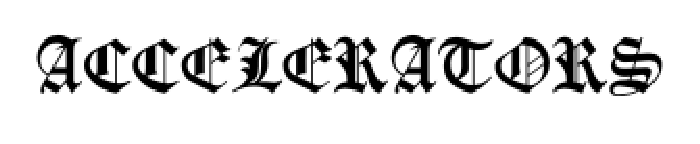
\includegraphics[width=.9\linewidth]{accelerator.eps} \\
\fontsize{29pt}{34pt}\selectfont \bf
  A Particle Beam Game \\
 A  Speed-of-Light Universe
}


\author{ 
\Large \bf
 Fran\c{c}ois~M\'eot \\
~ \\
Brookhaven National Laboratory \\
Collider-Accelerator Department \\
 Upton, LI, NY
}

\date{}

\maketitle



%\clearpage

%\tableofcontents




\clearpage

\fontsize{18pt}{24pt}\selectfont \bf


This course is an introduction  to the physics and technology of particle accelerators, 

\sid based on computer laboratory work during which will be manipulated
  charged  particle beams, short-lived particles, synchrotron light, etc.

\sid It will introduce  most types of existing particle  accelerators, their main optics and acceleration components, 

\sid it will introduce  the basic principles of beam dynamics and physics they lean on, 

\sid \textsl{via} numerical simulations using dedicated computer tools, 

\sid based  on computer simulation practice taken from real-life laboratory activities, hands-on. 

\sid Computer code develpoments will be part of the game.


~

This course also includes 

\sid conducting a project, from start to end, over the semester. Topics will be discussed and chosen early, 
during the first sessions. 

and it also is to be considered

\sid a forum for discussions and deeper insight, on whatever topic whenever desired, 
including further/unplanned code developments and simulations. 


~

During this semester, 

\sid students will run beam dynamics computer programs 

\sid manage the data they produce, 

\sid using  small sets of short, \textsl{ad hoc}, 
input data files and other data treatment computer tools which they will be provided. 
%and possibly further develop themselves.

\sid Beam dynamics findings from numerical simulations will be confronted with theoretical expectations,  

\sid in an interactive play between both~: experimentation regarding particle beams in accelerators and in accelerator 
components, and the underlying theory.

~

Purpose of the course~:  contribute preparing to 

\sid   the understanding of the physics and dynamics of charged particle beams, 

\sid  the understanding of the physics and functioning of various  accelerator types and components, 

\sid  the technics/methods/tools for the design of  particle accelerators. 

\bigskip

Running computer programs will allow achieving  a variety of goals~: 

\sid apply numerical methods to solve problems for which  analytical methods have prohibitive limitations, 

\sid produce  data from  numerical simulations, 

\sid analyze and understanding these data, 
 
\sid present and report results on appropriate media. 


\bigskip

This course will allow  reaching a level of  knowledge needed to thrive in the field of accelerator physics and technology, 
it will navigate and pick knowledge bricks through the following list, as time allows~: 

\sid cyclotron, transverse stability, CW acceleration~;

\sid synchro-cyclotron,  longitudinal stability,  pulsed acceleration~; 

\sid FFAG rings, strong focusing~;  

\sid pulsed synchrotron~; 

\sid storage rings including colliders, light sources,  insertion devices~; 

\sid particle collider~; 

\sid electrostatic accelerators~; 

\sid linear accelerators. 


The numerical experiments will address  beam physics and beam dynamics aspects as 

\sid beam guiding, focussing, acceleration, optical defects,

\sid non-linear beam dynamics and motion resonances, 

\sid  synchrotron radiation damping, 

\sid collective effects as space charge,

\sid capture and acceleration of short lived particle beams, 

\sid the production of synchrotron light,  Poynting vector, spectral brightness, 

\sid  polarization and other siberian snakes, 

\sid in-flight particle decay,

\sid  beam purification. 


As part of the computer simualtion building blocks, 
the course  will address the simulation of accelerator technology components as bending magnets, quadrupoles, 
non-linear lenses, accelerating cavities, beam monitoring.

As part of the computer simulation activities,  program development and debugging will be part of the lab time. 

\bigskip

In addition, and for the reason that this is what numerical simulations are,  
the course will  introduce to a wide variety of applied mathematics and numerical methods, from 
interpolation  to ODE solving to Fourier analysis. 

The course will introduce to popular software tools as  gnuplot (plotting),  latex (writing). 

\bigskip

\section*{Organization of the course}

A 2$\times$1h40  session 
will be organized in the following way~: 



\bigskip

Lecture notes will be provided \textsl{via} .pdf files produced under latex. Students are expected to turn in their 
computer lab time and home work assignments under the same environment. 
Preparation of lab time experiment sessions will be part of home work assignments.

 




This computer workshop is organized in the following way:


We will have **15** weeks together, two 1:40 sessions per week. 

The first **2** sessions will be organized in a particular way, aimed at 

(i) introducing -~briefly by necessity, $\bf 2\times $1:40hr this is short~- to the vast, and rich, world of accelerators

(ii) introducing to the computer game that will be played, Zgoubi. 

In order that no one fall asleep being bored by History -~a matter that we may have disliked at the primary school~\sid 
we will split the 1:40 session into the two topics.


A regular $\bf 2\times $1:40hr session will be organized in the following way:

presntation/introduction to the session topic and to the software tools (20~min.)~; computer simulations and data analysis (2h30). 

\sid  a bried review of the  underlying theoretical principles of the ``topic of the day'', 30$\sim$45 minutes. 
Their, it is assumed that essential knowledge is acquired prior to the lecture. 
Guidance, instruction and bibliography will be provided for that.

\sid  presntation/introduction to the session topic,  \textsl{ad hoc} software tools,  computer simulations
and data analysis planned.

~

Home work:

\bigskip

Only minor home work volume is foreseen. Essentially,

\sid prepare the next lectures  by reading a few scientific articles targetted on the subject

\sid Work on the semester project.



\clearpage

BACKUP SLIDES 


\addcontentsline{toc}{section}{\LARGE Backup slides}

\sethlcolor{blue!10!white}

\nib MULTIPLE-PASS : ~    \hl{1~up + 1~down}, ~ ~ \hl{3~up + 3~down}, ~ ~ \hl{5~up + 5~down}


\sethlcolor{yell60}


\nib MULTIPLE-PASS : ~    \hl{1~up + 1~down}, ~ ~ \hl{3~up + 3~down}, ~ ~ \hl{5~up + 5~down}

~

~

   \begin{tabular}{lcc}
\hline
{\cellcolor{yellow!50} Numb. of cavities/linac       } & No color & No color \\
\hline
   \end{tabular}




~

~

{
\setlength{\fboxsep}{0pt}%
\fbox{\Large \red $\begin{array}{l} \textrm{WEPMW027: ``The ERL-based Design of
   Electron-Hadron-Collider eRHIC''} \\
\textrm{WEPMW044: ``Start-to-End Simulation of eRHIC ERL''}
\end{array}$}
}

~

~
\raisebox{4.2ex}[0mm][0mm]{ \hspace{.37\linewidth} \LARGE \fcolorbox{white}{blue!10!white}{: EIC R\&D}}

~

\fontsize{29pt}{34pt}\selectfont

VOIVAOIV

leobjcf;

ncpeoi



~

~

{\Large \black
\hspace{.6\linewidth}\fcolorbox{black}{yellow!40!white}{$\begin{array}{c}\textrm{C. Dubbe} \\ \textrm{JLab}  \end{array}$}
}

\end{document}



The goal of this computer workshop is manyfold:

- an introduction to particle accelerators

- based  on computer simulation practice taken from real-life laboratory activities, 
 thus an introduction to accelerator physics and technology via ``the way that works'', hands-on

- an introduction to accelerator design methods

- and to dedicated computer simulation methods, and tools including their development

